\chapter{电负性、极性与分子间作用力}\label{ch:g11:polarity-and-cohesion}

壁虎沿着窗玻璃向上爬，只靠一只脚趾挂在玻璃上，
不用胶水，也没有吸盘。水分子 \ce{H2O} 比
硫化氢分子 \ce{H2S} 轻，但水在
\qty{100}{\celsius} 时沸腾，而硫化氢在低至
\qty{-60}{\celsius} 时仍是气体。两件事说的是同一件事：使分子彼此之间、
以及分子与其他物体之间的作用力。它们远比分子内的共价键弱，
但决定了物质在室温下是
气体、液体还是固体，也决定了
壁虎会不会掉下来。

\begin{recall}
共价键是由两个原子共用的一对电子；路易斯
结构表示成键电子对与孤电子对，而中心原子周围的
电子对决定分子的形状
（见\cref{ch:g10:lewis-and-shape}）。离子带有电荷；在离子固体中，
正、负离子相互吸引（见\cref{ch:g9:ions}）。
\end{recall}

\begin{omfigure}
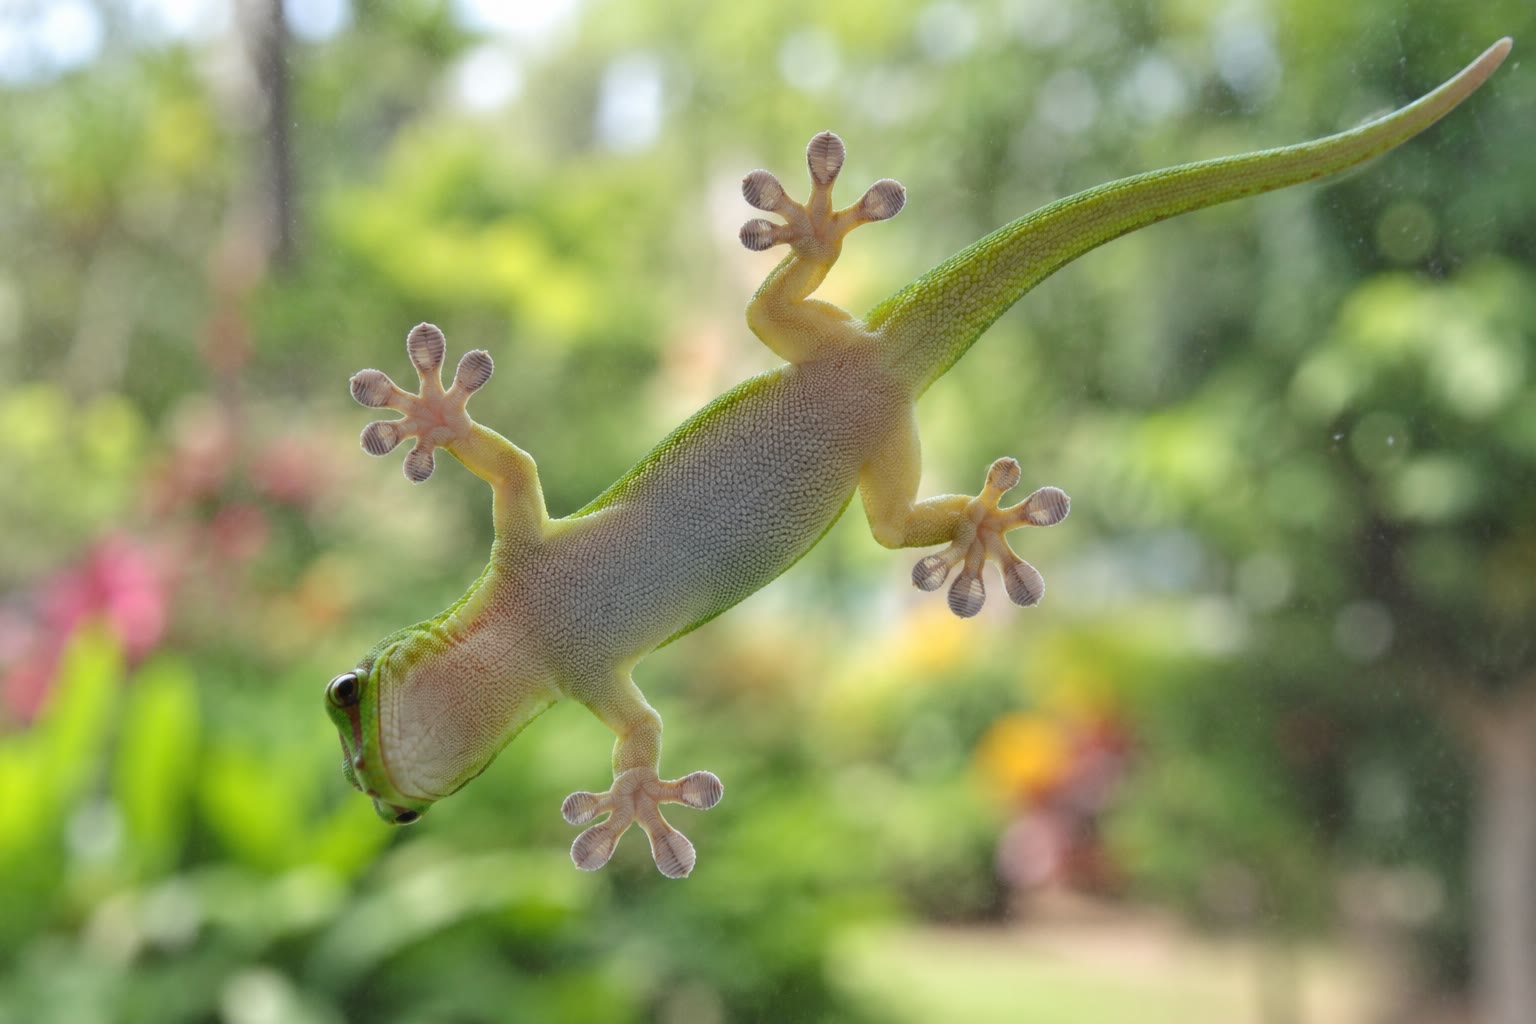
\includegraphics[width=0.5\linewidth]{images/book1/ai/g11-gecko-glass.jpg}

{\small 壁虎趴在玻璃板上：其趾垫依靠分子之间
的作用力附着。}
\end{omfigure}

\section{电负性}

\begin{definition}[电负性]\label{def:g11:polarity-and-cohesion:electronegativity}
元素的\emph{电负性}\index{电负性}，用来衡量该元素的原子在分子中
吸引所形成化学键中电子的能力强弱。它是
没有单位的数。在常用标度上，
其取值约从 0.8 到 4。
\end{definition}

\begin{omfigure}
% ledger: en:H, en:Li, en:Be, en:B, en:C, en:N, en:O, en:F, en:Na, en:Mg, en:Al, en:Si, en:P, en:S, en:Cl, en:K, en:Ca
\omperiodictable[upto=20, f block=false, cell=0.9cm, values={H/2.20,
  Li/0.98, Be/1.57, B/2.04, C/2.55, N/3.04, O/3.44, F/3.98, Na/0.93,
  Mg/1.31, Al/1.61, Si/1.90, P/2.19, S/2.58, Cl/3.16, K/0.82, Ca/1.00},
  highlight={F,O,N,Cl}]

{\small 前 20 号元素的电负性（鲍林标度；
未列出氦、氖和氩，它们在此不形成化学键）。
图中高亮显示的是电负性最大的四种元素。}
\end{omfigure}

\begin{proposition}[表中的变化规律]\label{prop:g11:polarity-and-cohesion:trends}
% ledger: en:F, en:Li, en:Cl, en:K
同一周期中，电负性从左到右增大，
同一族中从上到下减小。氟（3.98）是电负性最大的元素，
碱金属的电负性最小（锂 0.98，
钾 0.82）。
\end{proposition}

\begin{proof}
由表中数据可得：第 2 周期中，$0.98 < 1.57 < 2.04 < 2.55 < 3.04 <
3.44 < 3.98$；在 17 族中，氟 $3.98$ 高于氯
$3.16$；在 1 族中，$2.20$、$0.98$、$0.93$、$0.82$。（其原因
在本科一年级分册中有解释。）
\end{proof}

\begin{history}[鲍林标度，1932 年]
化学家莱纳斯·鲍林于
1932 年，根据不同原子间化学键的键能，建立了第一个电负性标度。该标度中
氟取值最大，本章所用的标度至今仍
以他的名字命名。
\end{history}

\section{极性键与极性分子}

\begin{definition}[极性键，部分电荷]\label{def:g11:polarity-and-cohesion:polar-bond}
两个电负性不同的原子之间的共价键是
一种\emph{极性键}\index{极性键}：共用电子对更靠近
电负性较大的原子。该原子带有较小的负
\emph{部分电荷}\index{部分电荷}，记作 $\delta^-$，另一原子则
带等量的正部分电荷，记作 $\delta^+$。
\end{definition}

\begin{proposition}[何时为极性键？]\label{prop:g11:polarity-and-cohesion:polar-bond}
% ledger: en:C, en:H, en:O, en:Na, en:Cl
由两个相同原子形成的化学键不是极性键。不同原子之间，
电负性之差越大，化学键的极性越强。作为经验规则，
电负性之差小于约 0.4 时（如
\ce{C-H}，$2.55 - 2.20 = 0.35$），视为非极性键。
电负性之差很大时（如钠与氯，$3.16 - 0.93 = 2.23$），
电子不再是共用，而是转移，该化合物为离子化合物。
\end{proposition}

\begin{proof}
在本阶段不加证明地承认：这由电负性的定义得出，
其中的阈值只是人为约定。
\end{proof}

\begin{definition}[极性分子与非极性分子]\label{def:g11:polarity-and-cohesion:polar-molecule}
若分子中正部分电荷的中心与负部分电荷的中心
不重合，则该分子称为\emph{极性分子}\index{极性分子}；
若两者重合，则该分子称为
\emph{非极性分子}\index{非极性分子}。
\end{definition}

\begin{method}[分子是否有极性？]\label{met:g11:polarity-and-cohesion:polar}
\begin{enumerate}
  \item 画出分子的路易斯结构，并确定分子的形状。
  \item 在极性键上标出 $\delta^+$ 和 $\delta^-$。
  \item 若不含极性键，则该分子为非极性分子。否则，
        看形状：若极性键围绕中心对称排列，
        则其作用相互抵消，分子为
        非极性分子；否则为极性分子。
\end{enumerate}
\end{method}

\begin{omfigure}
\begin{tikzpicture}[font=\small]
  % water
  \begin{scope}
    \node[aO] (o) at (0,0) {};
    \node[aH] (h1) at (-0.82,-0.6) {};
    \node[aH] (h2) at (0.82,-0.6) {};
    \begin{scope}[on background layer]
      \draw[bond] (o.center) -- (h1.center); \draw[bond] (o.center) -- (h2.center);
    \end{scope}
    \node[omThm] at (0,0.55) {$2\delta^-$};
    \node[omDef] at (-1.22,-0.5) {$\delta^+$};
    \node[omDef] at (1.22,-0.5) {$\delta^+$};
    \fill[omDef] (0,-0.6) circle (0.06);
    \fill[omThm] (0,0) circle (0.06);
    \draw[densely dotted, black!60] (-0.82,-0.6) -- (0.82,-0.6);
    \draw[<-, black!60] (0.08,-0.64) -- (1.55,-1.05) node[right, align=left,
      font=\footnotesize] {$\delta^+$ 的 \\中心};
    \node[align=center, anchor=north] at (0,-1.8) {水：折线形，\textbf{极性}};
  \end{scope}
  % carbon dioxide
  \begin{scope}[xshift=6cm]
    \node[aO] (o1) at (-1.15,0) {};
    \node[aC] (c) at (0,0) {};
    \node[aO] (o2) at (1.15,0) {};
    \begin{scope}[on background layer]
      \draw[bond, double, double distance=1.6pt] (o1.center) -- (c.center);
      \draw[bond, double, double distance=1.6pt] (c.center) -- (o2.center);
    \end{scope}
    \node[omThm] at (-1.15,0.55) {$\delta^-$};
    \node[omThm] at (1.15,0.55) {$\delta^-$};
    \node[omDef] at (0,0.55) {$2\delta^+$};
    \draw[->, omProp, thick] (-0.25,-0.45) -- (-1.0,-0.45);
    \draw[->, omProp, thick] (0.25,-0.45) -- (1.0,-0.45);
    \node[align=center, anchor=north] at (0,-1.8) {二氧化碳：直线形，\\
      \textbf{非极性}};
  \end{scope}
\end{tikzpicture}

{\small 在水中，折线形的结构使正部分电荷的中心（位于两个氢原子之间）
位于氧原子下方，因此水是极性分子。
在二氧化碳中，两个极性键的作用方向相反（见箭头），
相互抵消，电荷中心重合于
碳原子上。}
\end{omfigure}


\begin{example}[四种分子]\label{ex:g11:polarity-and-cohesion:four}
氯化氢 \ce{HCl} 含有一个极性键，是极性分子，其中氯原子带 $\delta^-$。
氨 \ce{NH3} 为三角锥形，含三个极性 \ce{N-H} 键，是极性分子，其中氮原子带 $\delta^-$。
甲烷 \ce{CH4} 中只有近似非极性的
\ce{C-H} 键，是非极性分子。四氯化碳 \ce{CCl4} 含有四个极性
\ce{C-Cl} 键，但它们分布在正四面体的顶点上，
相互抵消，因此该分子是非极性分子。
\end{example}

\section{范德瓦耳斯相互作用}

\begin{definition}[范德瓦耳斯相互作用]\label{def:g11:polarity-and-cohesion:van-der-waals}
称\emph{范德瓦耳斯相互作用}\index{范德瓦耳斯相互作用}为相邻分子之间的一种较弱的吸引作用，
它存在于所有分子之间，无论是否为极性分子：每个分子的电子
都在不断运动，某一瞬间分子中电荷分布的不均匀，会吸引
相邻分子中的相应电荷。在极性分子之间，
永久部分电荷还会带来一份额外的吸引
作用。
\end{definition}


\begin{proposition}[分子越大，吸引作用越强]\label{prop:g11:polarity-and-cohesion:size}
范德瓦耳斯相互作用随分子尺寸增大而增强，即
随分子中电子数的增多而增强；在结构相似的分子之间，
较大的分子具有较高的熔点和沸点。
\end{proposition}

\begin{proof}
在本阶段不加证明地承认：电子云较大的分子更容易变形，因此
其瞬间电荷更大，
且与相邻分子的接触更多。
\end{proof}

\begin{example}[卤素]\label{ex:g11:polarity-and-cohesion:halogens}
% ledger: bp:F2, bp:Cl2, bp:Br2, bp:I2 (K values converted)
\ce{F2}、\ce{Cl2}、\ce{Br2}、\ce{I2} 这些分子都是非极性分子，并且
分子越来越大，它们的沸点也随之升高：
\qty{-188}{\celsius}、\qty{-34}{\celsius}、\qty{59}{\celsius} 和
\qty{184}{\celsius}。常温下，氟和氯为
气体，溴为液体，碘为固体。
\end{example}

\begin{remark}[壁虎]\label{rem:g11:polarity-and-cohesion:gecko}
单个范德瓦耳斯相互作用非常微弱，但它们可以累加。壁虎的
趾垫上布满致密的微观绒毛，
每根绒毛又分出更细的末端，这些末端与玻璃
足够靠近，使范德瓦耳斯相互作用能在很大的总面积上发挥作用。
\end{remark}

\section{氢键}

\begin{definition}[氢键]\label{def:g11:polarity-and-cohesion:hydrogen-bond}
称\emph{氢键}\index{氢键}为一种吸引作用，它存在于
与电负性很大的原子（氮、氧或氟）相连的氢原子之间，
（该氢原子带有明显的 $\delta^+$）与另一个氮、氧或氟原子的
孤电子对之间，后者常位于相邻分子中。氢键用虚线表示，
涉及的三个原子几乎
位于一条直线上。
\end{definition}

\begin{omfigure}
\begin{tikzpicture}[font=\small]
  % central water molecule and four neighbours, H-bonds dashed
  \newcommand{\water}[4]{% name, x, y, rotation
    \begin{scope}[shift={(#2,#3)}, rotate=#4]
      \node[aO] (#1o) at (0,0) {};
      \node[aH] (#1a) at (-0.6,-0.45) {};
      \node[aH] (#1b) at (0.6,-0.45) {};
    \end{scope}
    \begin{scope}[on background layer]
      \draw[bond] (#1o.center) -- (#1a.center); \draw[bond] (#1o.center) -- (#1b.center);
    \end{scope}}
  \water{m}{0}{0}{0}
  \water{p}{-1.62}{-1.215}{0}
  \water{q}{1.62}{-1.215}{0}
  \water{r}{-1.435}{1.435}{-8.13}
  \water{s}{1.435}{1.435}{8.13}
  % H-bonds: m's H to p's O and q's O; r's and s's H to m's O
  \draw[dashed, omDef, thick] (ma) -- (po);
  \draw[dashed, omDef, thick] (mb) -- (qo);
  \draw[dashed, omDef, thick] (rb) -- (mo);
  \draw[dashed, omDef, thick] (sa) -- (mo);
\end{tikzpicture}

{\small 液态水中，一个水分子周围的氢键（虚线）：
其两个氢原子与两个相邻分子的氧原子形成氢键，
其氧原子上的两个孤电子对接收另外两个分子的
氢原子。}
\end{omfigure}


\begin{example}[乙醇与丙烷]\label{ex:g11:polarity-and-cohesion:ethanol}
% ledger: bp:C2H5OH, bp:C3H8 (K values converted)
乙醇 \ce{CH3-CH2-OH}（\qty{46.0}{g/mol}）与丙烷，
\ce{CH3-CH2-CH3}（\qty{44.0}{g/mol}）的分子大小几乎相同。然而，
乙醇的沸点为 \qty{78}{\celsius}，丙烷的沸点为
\qty{-42}{\celsius}。乙醇分子含有 \ce{O-H} 基团，
彼此之间能形成氢键；丙烷分子则不能。
\end{example}

\section{固体与液体的内聚力}

\begin{definition}[分子晶体]\label{def:g11:polarity-and-cohesion:molecular-solid}
称\emph{分子晶体}\index{分子晶体}为由分子构成的固体，其中分子
借范德华相互作用彼此吸引，并在可能时借氢键相互结合。
冰、固态碘和蔗糖都属于
分子晶体。
\end{definition}

\begin{proposition}[内聚与相变]\label{prop:g11:polarity-and-cohesion:cohesion}
物质粒子之间的吸引作用越强，
其熔化温度和沸腾温度越高。按作用力由弱到强排列为：
范德华相互作用、氢键，以及离子晶体中离子之间的
吸引作用。
\end{proposition}

\begin{proof}
在本阶段不加证明地承认：熔化与沸腾都要克服这些
吸引作用使粒子彼此分离，需要更多的能量，因此
当吸引作用较强时，所需温度更高。
\end{proof}

\begin{example}[三种固体]\label{ex:g11:polarity-and-cohesion:three}
% ledger: mp:NaCl, mp:water
氯化钠是离子晶体，熔化温度为 \qty{801}{\celsius}；冰
借氢键结合，熔化温度为 \qty{0}{\celsius}；固态甲烷仅借
小分子之间的范德华相互作用维系，熔化温度远低于
\qty{-150}{\celsius}。
\end{example}

\begin{omfigure}
\begin{tikzpicture}
\begin{axis}[width=0.6\linewidth, height=7cm, xmin=1.7, xmax=5.3,
    ymin=-190, ymax=120, xtick={2,3,4,5}, xlabel={周期},
    ylabel={沸腾温度（\si{\celsius}）}, axis lines*=left,
    ymajorgrids, grid style={gray!20}, tick label style={font=\small},
    label style={font=\small},
    legend style={font=\small, at={(1.02,0.5)}, anchor=west, draw=none},
    legend cell align=left]
  % ledger: bp:CH4, bp:SiH4, bp:GeH4, bp:NH3, bp:PH3, bp:AsH3, bp:SbH3, bp:H2O, bp:H2S, bp:H2Se, bp:HF, bp:HCl, bp:HBr, bp:HI (K values converted to degC)
  \addplot[thick, mark=*, black!70] coordinates {(2,-162.2) (3,-112) (4,-88.1)};
  \addplot[thick, mark=square*, omMeth] coordinates {(2,-33.4) (3,-87.8) (4,-62.5) (5,-18.4)};
  \addplot[thick, mark=triangle*, mark size=3pt, omThm] coordinates {(2,100.0) (3,-60.3) (4,-41.3)};
  \addplot[thick, mark=diamond*, mark size=3pt, omDef] coordinates {(2,19.6) (3,-85.1) (4,-66.4) (5,-35.1)};
  \legend{14 族（\ce{CH4} \dots）、15 族（\ce{NH3} \dots）、
    16 族（\ce{H2O} \dots）、17 族（\ce{HF} \dots）}
  \node[font=\footnotesize, anchor=west] at (axis cs:2.05,100) {\ce{H2O}};
  \node[font=\footnotesize, anchor=west] at (axis cs:2.05,19.6) {\ce{HF}};
  \node[font=\footnotesize, anchor=west] at (axis cs:2.05,-33.4) {\ce{NH3}};
  \node[font=\footnotesize, anchor=north west] at (axis cs:2.05,-166) {\ce{CH4}};
\end{axis}
\end{tikzpicture}

{\small 氢与 14 至 17 族元素形成的化合物的沸腾温度。
在同一族中，沸腾温度随分子增大而升高，
但 15、16 和 17 族的第一个成员例外，其沸腾温度
高得多：氨、水和氟化氢能够形成氢键。（
资料未给出数值处不绘点。）}
\end{omfigure}

\begin{remark}[冰与雪]\label{rem:g11:polarity-and-cohesion:ice}
冰中，每个水分子都与四个相邻分子形成氢键，呈
由六元环组成的开放网络。这一网络留出的空隙比
液态水更多，而液态水中氢键不断断开、重新形成。冰的
密度小于水，因此会漂浮。雪晶的六重对称性
反映了网络中的六元环。
\end{remark}

\begin{omfigure}
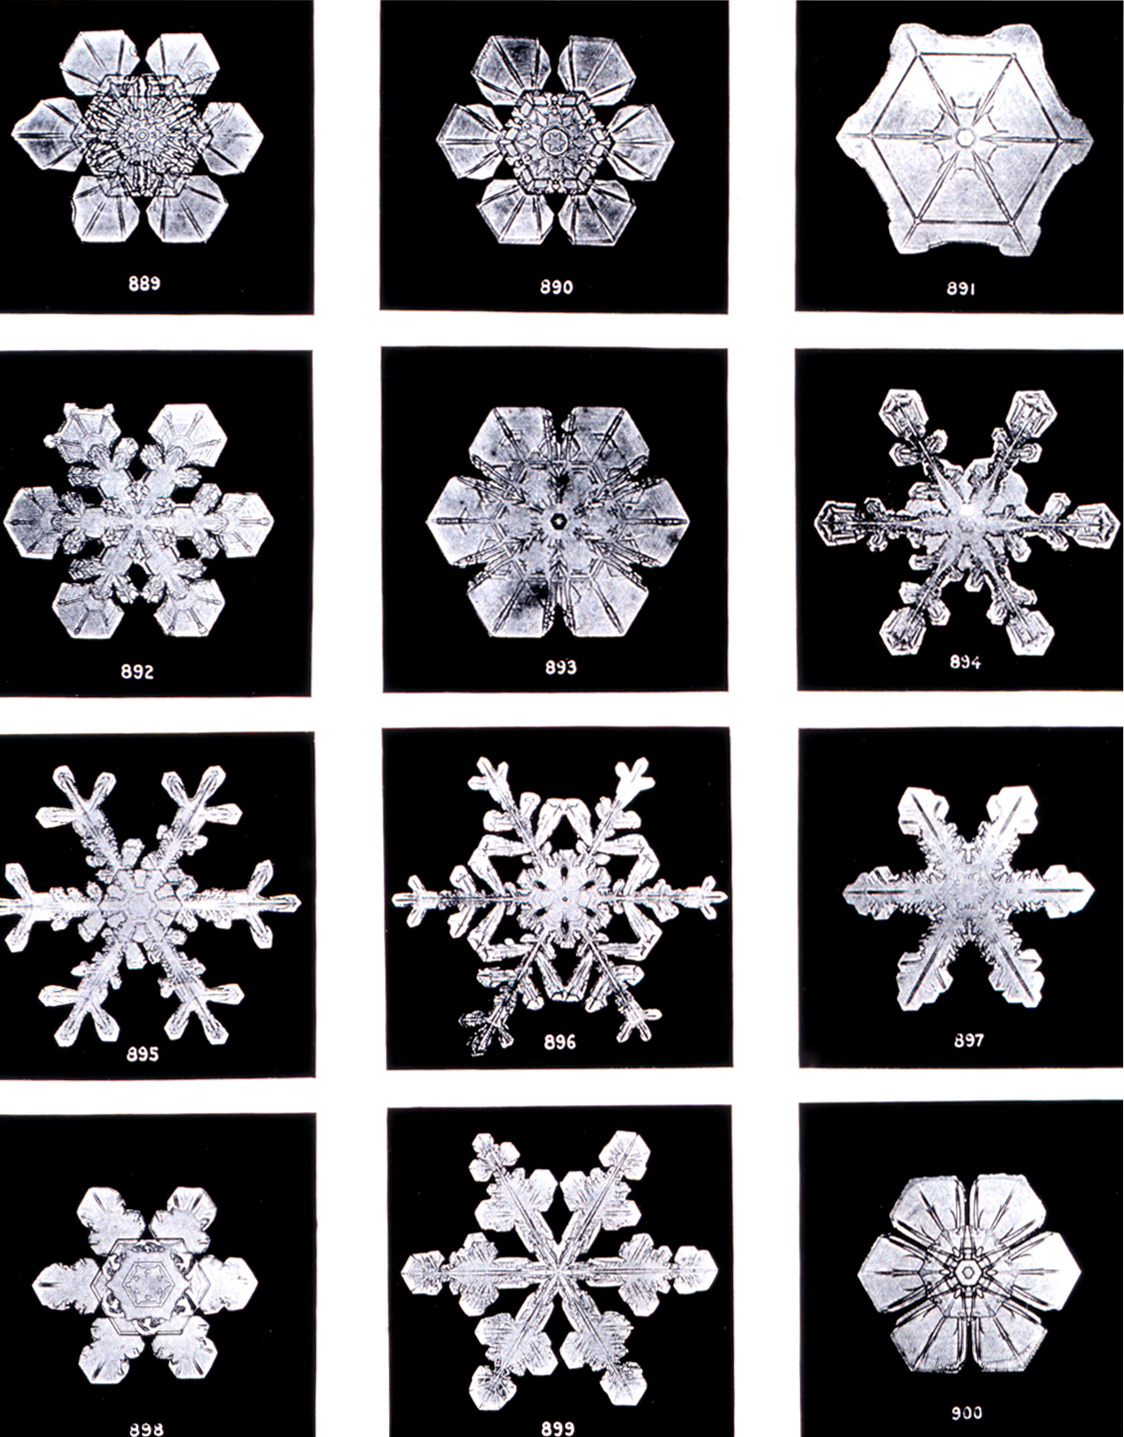
\includegraphics[width=0.36\linewidth]{images/book1/snowflakes.jpg}

{\small 威尔逊·本特利于 1900 年代初拍摄的雪晶：
每一片都有六个分支。}
\end{omfigure}

\section{练习}


\begin{exercise}[$\star$]\label{exo:g11:polarity-and-cohesion:1}
在 \ce{H-Cl}、\ce{O-H} 和 \ce{C-O} 这些键中，哪一个原子
带有部分电荷 $\delta^-$？请利用电负性表。
\end{exercise}

\begin{exercise}[$\star$]\label{exo:g11:polarity-and-cohesion:2}
下列键中，哪些是极性键：\ce{H-H}、\ce{C-H}、\ce{O-H}、\ce{N-H}、
\ce{Cl-Cl}、\ce{C-Cl}？请分别给出
各键的电负性之差。
\end{exercise}

\begin{exercise}[$\star$]\label{exo:g11:polarity-and-cohesion:3}
在每组元素中，电负性更大的是哪一种：氮或
磷；氧或硫；碳或氮；钠或镁？
每组各体现了表中的哪一种变化趋势？
\end{exercise}

\begin{exercise}[$\star$]\label{exo:g11:polarity-and-cohesion:4}
\ce{CH4}、\ce{NH3}、\ce{H2O} 和 \ce{HCl} 中，哪些能在
自身分子之间形成氢键？请说明理由。
\end{exercise}

\begin{exercise}[$\star$]\label{exo:g11:polarity-and-cohesion:5}
甲烷的非极性分子之间是否存在
吸引作用？为什么甲烷在室温下仍是气体？
\end{exercise}

\begin{exercise}[$\star\star$]\label{exo:g11:polarity-and-cohesion:6}
判断下列各分子是否为极性分子：二氯甲烷 \ce{CH2Cl2}
（四面体形）、四氯化碳 \ce{CCl4}、氨 \ce{NH3}、二氧
化碳 \ce{CO2}、三氟化硼 \ce{BF3}（平面三角形，
硼位于中心）。
\end{exercise}

\begin{exercise}[$\star\star$]\label{exo:g11:polarity-and-cohesion:7}
在甲醇 \ce{CH3-OH} 中，哪个氢原子可以提供
形成氢键？哪个原子可以接受？甲醇分子与水分子之间能否
相互形成氢键？请画出一例。
\end{exercise}

\begin{exercise}[$\star\star$]\label{exo:g11:polarity-and-cohesion:8}
请解释为什么沸点按 \ce{CH4} <
\ce{SiH4} < \ce{GeH4} 的顺序依次升高。
\end{exercise}

\begin{exercise}[$\star\star$]\label{exo:g11:polarity-and-cohesion:9}
在氢化物沸点图表中，哪一族
的首个成员没有出现异常数值？为什么？
\end{exercise}

\begin{exercise}[$\star\star$]\label{exo:g11:polarity-and-cohesion:10}
% ledger: en:H, en:Cl, en:Br, en:I, bp:HCl, bp:HBr, bp:HI
键 \ce{H-Cl}、\ce{H-Br}、\ce{H-I} 的极性越来越小（
氯、溴和碘的电负性分别为 3.16、2.96
和 2.66），但沸点却升高：\qty{-85}{\celsius}，
\qty{-66}{\celsius}、\qty{-35}{\celsius}。哪种相互作用起主导作用，
为什么？
\end{exercise}

\begin{exercise}[$\star\star$]\label{exo:g11:polarity-and-cohesion:11}
室温下，氯呈气态，碘呈固态，尽管两者
都由非极性分子 \ce{X2} 构成。请解释。
\end{exercise}

\begin{exercise}[$\star\star\star$]\label{exo:g11:polarity-and-cohesion:12}
% ledger: bp:C2H5OH, bp:CH3OCH3, bp:C3H8
乙醇 \ce{CH3-CH2-OH}、甲氧基甲烷 \ce{CH3-O-CH3} 和丙烷
\ce{CH3-CH2-CH3} 的摩尔质量几乎相同，它们的沸点依次为
\qty{78}{\celsius}、\qty{-25}{\celsius} 和 \qty{-42}{\celsius}。
下列哪些是极性分子？哪些在自身分子间形成氢键？
请解释这一顺序。
\end{exercise}

\begin{exercise}[$\star\star\star$]\label{exo:g11:polarity-and-cohesion:13}
在冰中，每个水分子与四个近邻通过氢键相连，
形成开放的网络；在液态水中，网络不断断裂，
并部分塌缩。请解释冰为什么漂浮在水上。为什么这一点对
冰冻湖泊中的鱼类很重要？
\end{exercise}

\begin{exercise}[$\star\star\star$]\label{exo:g11:polarity-and-cohesion:14}
按熔点由低到高排列，并根据
粒子之间的吸引作用说明理由：氯化钾 \ce{KCl}、冰
\ce{H2O}、固态甲烷 \ce{CH4}。
\end{exercise}

\begin{exercise}[$\star\star\star$]\label{exo:g11:polarity-and-cohesion:15}
% ledger: en:F, en:O, bp:HF, bp:H2O
氟的电负性比氧大，因此 \ce{H-F} 键
比 \ce{O-H} 键更具极性。但水在 \qty{100}{\celsius} 沸腾，
而氟化氢在 \qty{20}{\celsius} 沸腾。数一数
每个分子能提供的氢原子数，以及能接受的孤电子对数，
并加以解释。
\end{exercise}

\section{问题：为什么水在 \texorpdfstring{\qty{100}{\celsius}}{100 摄氏度}沸腾？}

\begin{problem}[{周末问题——若不存在氢键，水会在
什么温度下沸腾？}]
\label{pb:g11:polarity-and-cohesion:1}
% ledger: en:H, en:O, en:S, en:Se, bp:H2O, bp:H2S, bp:H2Se, bp:CH4, bp:SiH4, bp:GeH4, bp:HCl, bp:HBr, bp:HF, bp:NH3, bp:PH3, bp:AsH3
氧、硫和硒位于周期表中的同一族，三者
均可与氢形成化合物：\ce{H2O}、\ce{H2S}、\ce{H2Se}。在
同族氢化物中，沸点通常随
分子的大小增加而升高。水打破了这一规律，偏离了多少？

\medskip
\noindent\textbf{第一部分——三个分子。}
\begin{enumerate}
  \item 画出 \ce{H2O}、\ce{H2S} 和 \ce{H2Se} 的路易斯结构。
        它们为什么相似？
  \item 计算它们的摩尔质量。
  \item 计算各键的电负性之差：
        \ce{O-H}、\ce{S-H} 和 \ce{Se-H}（氧 3.44，硫 2.58，
        硒 2.55，氢 2.20）。哪些键明显具有极性？
  \item 这三种分子的形状如何？它们是否为极性分子？
  \item 数一数每个分子的电子数。哪种分子间的
        范德瓦耳斯相互作用最强？
\end{enumerate}

\medskip
\noindent\textbf{第二部分——氢键。}
\begin{enumerate}[resume]
  \item 三种化合物中，哪一种的分子之间
        能形成氢键？其他两种为什么不能？
  \item 一个水分子最多可以参与
        多少个氢键？请画出它们。
  \item 在液态中，哪些相互作用
        使硫化氢分子结合在一起？
\end{enumerate}

\medskip
\noindent\textbf{第三部分——变化趋势。}
\begin{enumerate}[resume]
  \item 硫化氢在 \qty{212.9}{K} 沸腾，硒化氢在
        \qty{-41.3}{\celsius} 沸腾。请用摄氏度表示前者
        （$\theta = T - 273.15$）。
  \item 从第 3 周期（\ce{H2S}）到第 4 周期（\ce{H2Se}），
        沸点升高了多少？
  \item 为什么会升高？
  \item 假设从第 2 周期到第 3 周期的升高量相同，
        那么“正常”的 \ce{H2O} 会在什么温度下沸腾？
  \item 用第 14 族检验这一方法：\ce{SiH4} 的沸点为
        \qty{-112}{\celsius}，\ce{GeH4} 的沸点为 \qty{-88.1}{\celsius}。
        预测 \ce{CH4} 的沸点，并与实际值
        \qty{-162}{\celsius} 比较。外推是否精确？
  \item 对第 17 族做同样的计算（\ce{HCl} \qty{-85.1}{\celsius}，
        \ce{HBr} \qty{-66.4}{\celsius}），并与 \ce{HF} 的
        \qty{19.6}{\celsius} 比较。
\end{enumerate}

\medskip
\noindent\textbf{第四部分——差距。}
\begin{enumerate}[resume]
  \item 水的实际沸点为 \qty{100}{\celsius}。实际值与
        外推值之间的差距有多大？
  \item 对氨做同样的计算，所用数据为 \ce{PH3} \qty{-87.8}{\celsius} 和
        \ce{AsH3} \qty{-62.5}{\celsius}；氨的实际沸点为
        \qty{-33.4}{\celsius}。
  \item 将水、氟化氢和氨按差距大小排序，
        并通过统计氢键的数目解释这一排序。
  \item 若没有氢键，室温下水会是固体、液体还是气体？
        这对地球意味着什么？
  \item 为什么第 12 题的答案只是一个估计值？
  \item 给出最终答案：没有氢键时，水大约在多少温度下
        沸腾？
\end{enumerate}
\end{problem}
